\chapter{Lepton Flavour in the Standard Model and Beyond}\label{chapter1}

\begin{markdown}
---

+ This is the first chapter. It should softly introduce concepts like particles, particle families, the Standard Model, lepton flavour.
+ Historical context, motivation
 + Why/how was the first CLFV experiment conducted?

Sindrum II: what do they start with?
 - Generation mixing in neutrino oscillations


---
\end{markdown}

%Something like
The Standard Model is the theory at the heart of modern high energy physics. It describes the interactions between elementary particles and allows physicists to predict the outcome of interactions and decays to a previously unattainable precision. Little evidence so far has been able to contradict the formulation of the Standard Model, despite many fundamental questions remaining unanswered, such as the nature of dark matter, the reason for the matter-antimatter asymmetry in the universe, or the existence of exactly three generations of leptons and quarks.


\section{Historical context}
% Take a trip down muon/LFV memory lane
% Is the muon discovery history required?
% "you should write to make the topic clear to a reader who has not spent most of the last three years thinking about it."
% -> Need to explain what a muon is at some point I guess

\begin{figure}
    \centering
    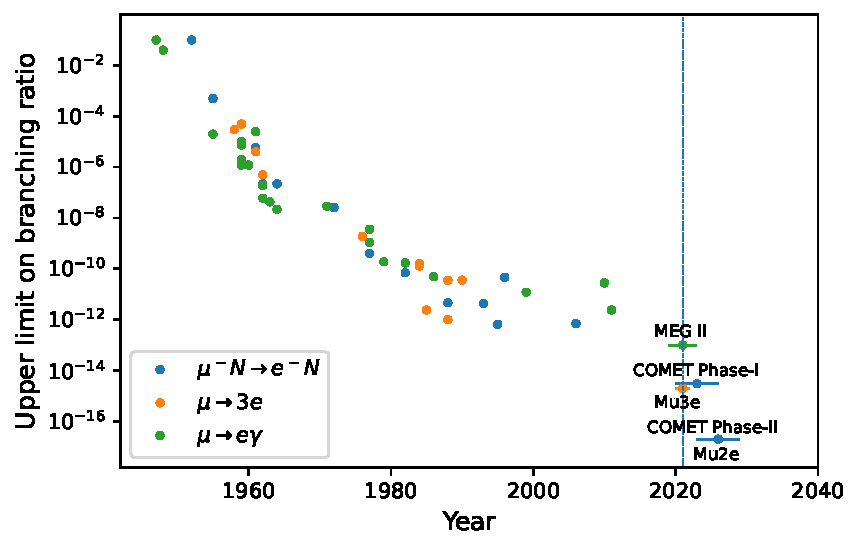
\includegraphics{chapter1/clfv_upper_limit.pdf}
    \caption{90\%-confidence upper limit on the branching ratio of three charged lepton flavour-violating processes over time. The past data points were tabulated in~\cite{BERNSTEIN201327}. Future data points are the expected sensitivities quoted in the MEG II~\cite{Baldini2018}, Mu3e~\cite{ARNDT2021165679}, COMET Phase-I~\cite{the_comet_collaboration_comet_2020} and Mu2e~\cite{osti_1172555} design reports.}
    \label{fig:clfv_upper_limit}
\end{figure}

The search for Lepton Flavour Violation started in 19XX with John Doe's experiment~\cite{doe}.

\section{Recent related measurements}
\hl{Recent results and implications: g-2, LHCb, neutrinos}

\cite{PhysRevLett.126.141801} % g-2

\cite{lhcbcollaboration2021test} % lhc-b R_K


%See Chapter~\ref{chapter2}, read~\cite{goodfellow_generative_2014}.\\
%The smooth boi can be seen on Fig.~\ref{subfig:smooth_boi}, and the outlined boi on %Fig.~\ref{subfig:smooth_boi}. The whole figure is Fig.~\ref{fig:my_label}.
%
%A derivative:
%$$\diff{x}{y} = 2\pi x y$$
%Insane!
%
%And here we typeset COMET in smallcaps: \COMET. This \acrshort{COMET} is an \emph{acronym}. %You can click it to see what it means.
%
%\begin{figure}
%    \centering
%    \subfloat[A smooth boi]{
%    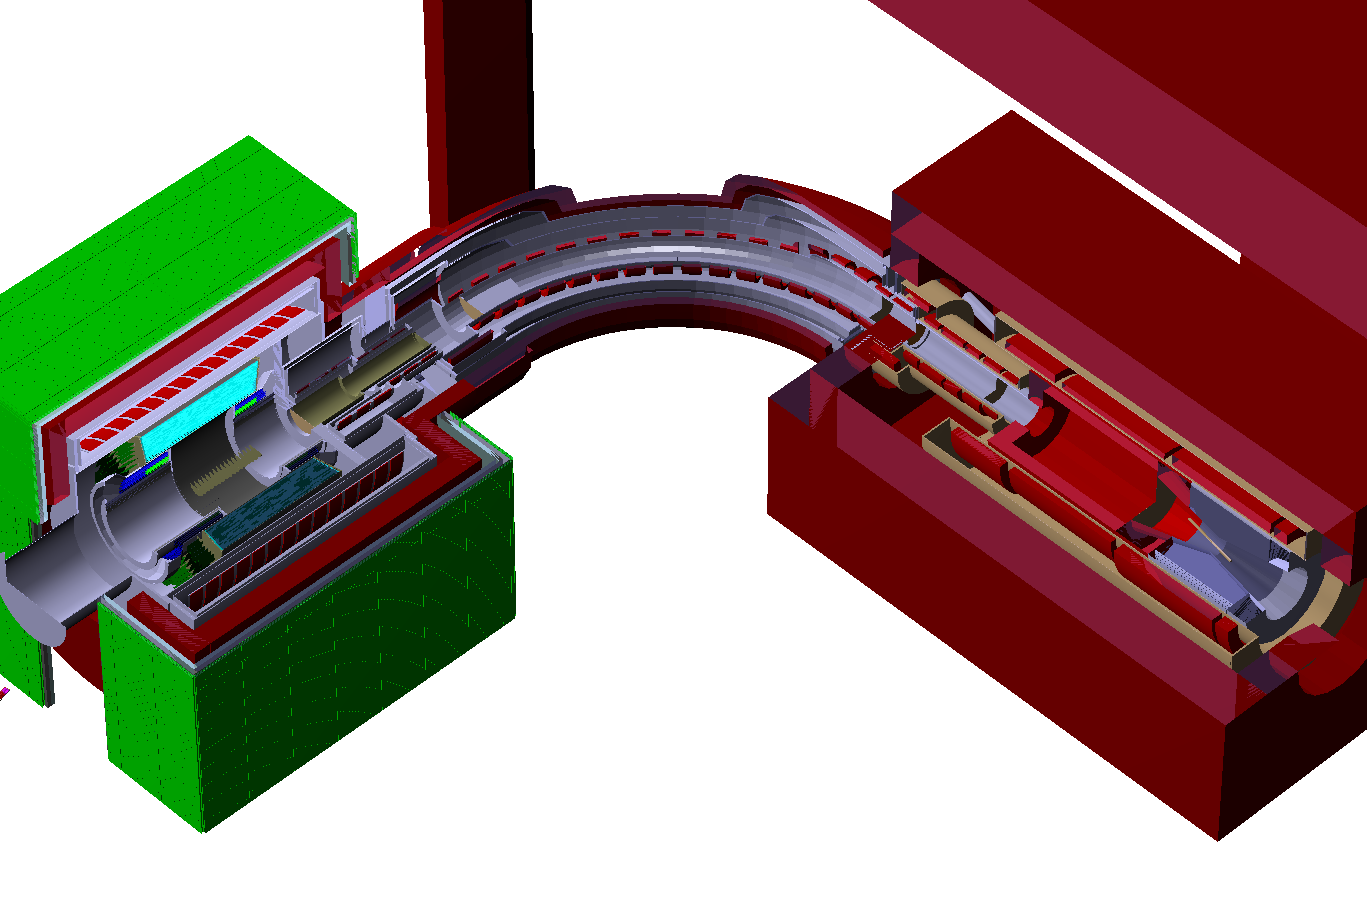
\includegraphics[width=0.5\textwidth]{viewer_smooth.png}
%    \label{subfig:smooth_boi}
%    }
%    \subfloat[An outlined boi]{
%    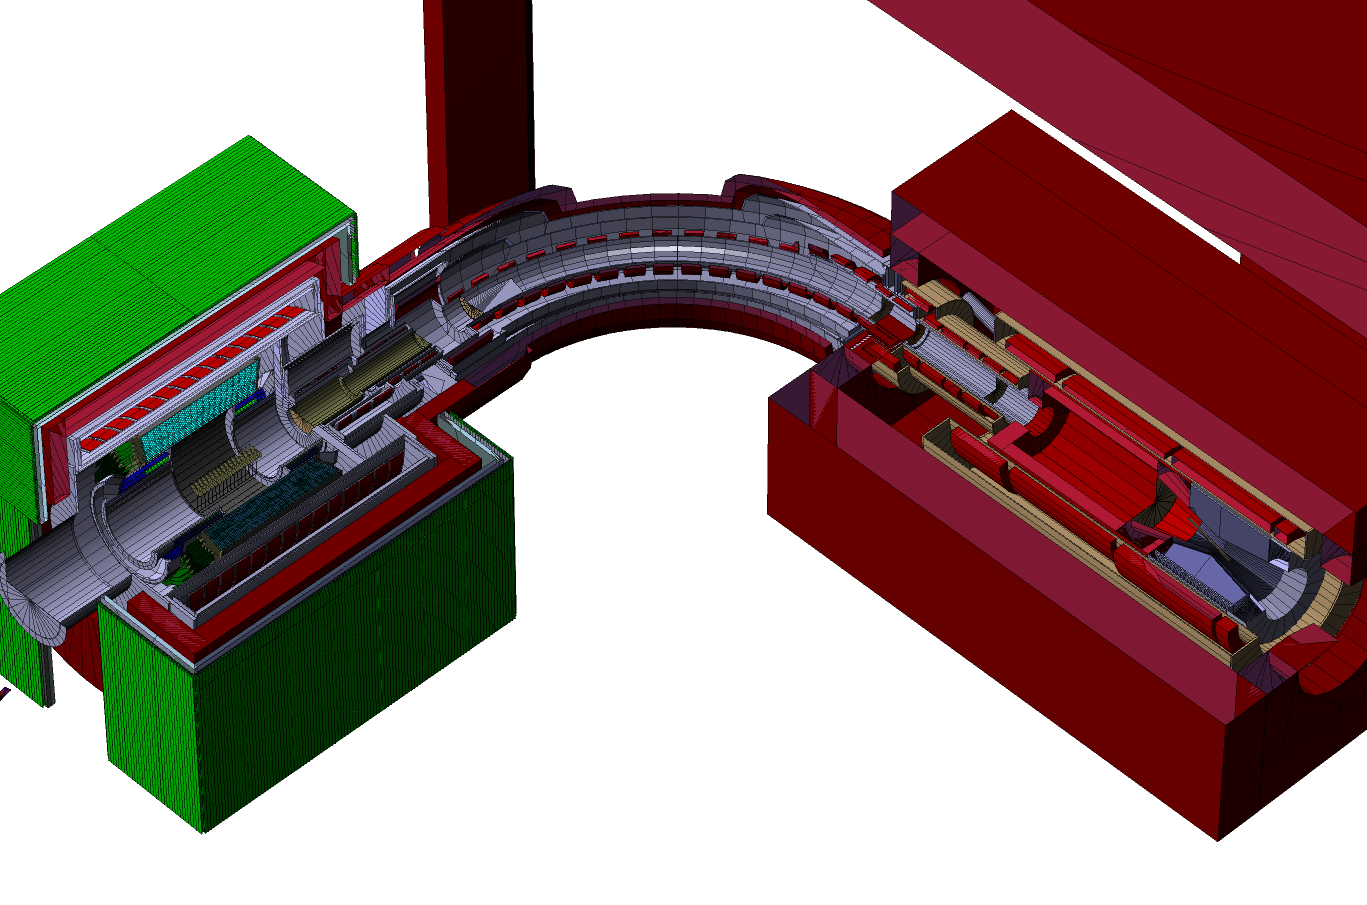
\includegraphics[width=0.5\textwidth]{viewer_outline2.png}
%    \label{subfig:outlined_boi}
%    }
%    \caption{Phase-I cutaway geometries.}
%    \label{fig:my_label}
%\end{figure}
%
%Here we cite the COMET TDR~\cite{the_comet_collaboration_comet_2020} and the upper limit on %the branching ratio of $\mu^- + \textrm{Al} \rightarrow e^- + \textrm{Al}$, $7\times %10^{-13}$, by the SINDRUM-II experiment~\cite{Bertl:2006up}.
